\documentclass[11pt,a4paper]{article}
\usepackage[margin=2.6cm]{geometry}
\usepackage[T1]{fontenc}
\usepackage{lmodern}
\usepackage[letterspace=180]{microtype}
\usepackage{booktabs}
\usepackage{amsmath}
\usepackage{parskip}
\usepackage{xcolor}
\usepackage{tikz}
\usepackage{pgfplots}
\pgfplotsset{compat=1.18}
\usepackage[most]{tcolorbox}
\usepackage{titlesec}
\usepackage{caption}

\definecolor{bcnavy}{RGB}{24,38,68}
\definecolor{bcgold}{RGB}{198,160,74}
\definecolor{bcteal}{RGB}{23,110,120}
\definecolor{bcgrey}{RGB}{95,95,95}

\titleformat{\section}{\bfseries\large\color{bcnavy}}{\thesection.}{0.6em}{}
\titleformat{\subsection}{\bfseries\color{bcteal}}{}{0em}{}
\captionsetup{font={footnotesize},labelformat=empty,textfont={color=bcgrey}}
\newcommand{\tabnote}[1]{\begin{center}\begin{minipage}{0.92\textwidth}
  \footnotesize\color{bcgrey}#1\end{minipage}\end{center}}

\begin{document}

% ---------------------------------------------------------------- cover
\begin{titlepage}
\centering
\vspace*{3.2cm}

\begin{tikzpicture}
  \fill[bcnavy] (0,0) rectangle (5,5);
  \node[bcgold] at (2.42,2.95)
    {\fontsize{44}{44}\selectfont\rmfamily B\hspace{-0.45em}\raisebox{-0.28ex}{C}};
  \node[bcgold] at (2.5,1.35)
    {\footnotesize\rmfamily\textls{BAYESIAN CAPITAL}};
  \fill[bcgold] (2.5,0.95) circle (0.035);
\end{tikzpicture}

\vspace{1.6cm}
{\color{bcnavy}\rule{7cm}{0.6pt}}

\vspace{0.9cm}
{\LARGE\bfseries\color{bcnavy} The Book on Verified Fills\par}
\vspace{0.35cm}
{\large\color{bcnavy} A fresh optimisation from first principles, the ten-name
ranking,\\ and what goes into the book\par}

\vspace{0.9cm}
{\color{bcgold}\rule{7cm}{1.0pt}}

\vspace{1.5cm}
{\bfseries Bayesian Capital}\\[0.2cm]
{\color{bcgrey} Systematic Trading Research}\\[0.9cm]
{\itshape\color{bcgrey} Internal document --- strictly confidential}\\[0.3cm]
{\color{bcgrey} 9 August 2026}
\vfill
\end{titlepage}

% ---------------------------------------------------------------- header
\begin{center}
{\Large\bfseries\color{bcnavy} The Book on Verified Fills}\\[0.15cm]
{\color{bcnavy} A fresh optimisation from first principles, the ten-name ranking,
and what goes into the book}\\[0.25cm]
{\small\color{bcgrey} Bayesian Capital --- Systematic Trading Research
\;$\bullet$\; TSM $\cdot$ VRT $\cdot$ VST $\cdot$ RKLB $\cdot$ MU
$\,\vert\,$ GM $\cdot$ VLO $\cdot$ CF $\cdot$ NVDA $\cdot$ AVGO\\
Back-test window 1 Apr 2024 -- 7 Aug 2026 ($\approx$2.35 years)
\;$\bullet$\; \$1{,}000{,}000 per name, two tranches of \$500{,}000}
\end{center}
\vspace{0.1cm}
{\color{bcnavy}\hrule height 0.8pt}
\vspace{0.5cm}

\section{Overview}

This note records a deliberate restart. The workbook's own return cells count
same-day round trips that daily bars cannot order, so the first job was an honest
profit basis; the second was to re-run parameter optimisation from the top on that
basis, with everything learned this cycle about why past searches failed; the third
was to put five candidate names through the identical instrument and rank all ten
for admission to the book.

The instrument, used identically everywhere: the validated Python replica of the
Model sheets (reproduces the live workbook's cached results to the digit on all
five names), the corrected \emph{residual} OU sigma, and \textbf{verified fills} ---
a same-day round trip is kept only where the 5-minute bars (587 of 591 sessions)
prove the low reached the bid before the high reached the target. One blade
decides everything: fit on the first half only, boundary 23 May 2025, freeze, score
the second half. No multi-fold slicing --- with 30--120 fills per half per name, a
single split is the only cut of this data whose verdicts stand on real samples.

\section{The honest baseline}

Verified fills roughly third the sheet's figures. This, not the sheet, is the
planning basis:

\begin{center}
\begin{tabular}{lrrrrr|r}
\toprule
 & TSM & VRT & VST & RKLB & MU & book \\
\midrule
sheet return cell   & 145\% & 242\% & 265\% & 525\% & 178\% & --- \\
\textbf{verified, full sample} & \textbf{56\%} & \textbf{58\%} & \textbf{50\%}
  & \textbf{161\%} & \textbf{65\%} & \textbf{84.8\%/yr} \\
\bottomrule
\end{tabular}
\end{center}

\tabnote{Annualised. Book is the held construction: equal capital, each name
compounding independently, never rebalanced between names.}

\section{Re-fitting is retired --- three independent instruments agree}

\textbf{The price process has no drift to track.} The Kalman filter's noise scales
have an exact likelihood on prices (63--126 daily observations per window, against
6--25 trades for the P\&L objective). Rolling maximum-likelihood fits stepped
monthly are homogeneous across the whole sample: every likelihood-ratio test
accepts a single parameter vector ($p = 0.42$--$0.98$), including across the
Jan--Apr 2025 AI drawdown. The market's monthly variation is real but enters the
model through the daily range, day by day, faster than any refit could.

\textbf{Fresh fits do not transport.} Two searches, both better-posed than
anything run before, both fitted on the train half against the verified robust
objective and scored frozen on the tested half:

\begin{itemize}
  \item \textbf{Variant A (8-dim).} The model is exactly invariant under
        $(\lambda,\varphi_L,\psi,k)\to(c\lambda,c\varphi_L,c\psi,k/c)$ --- the old
        10-dimensional search carried a pure flat direction. $\lambda$ is fixed
        at 1 with zero loss of expressiveness; ou\_W frozen.
  \item \textbf{Variant B (6-dim).} The filter pinned at its train-half maximum
        likelihood estimate; only the six policy knobs searched.
\end{itemize}

\begin{center}
\begin{tabular}{lrrr}
\toprule
tested half & deployed (frozen) & A & B \\
\midrule
TSM  & \textbf{80.7\%} & 58.4\% & 76.4\% \\
VRT  & \textbf{157.4\%} & 63.3\% & 50.0\% \\
VST  & \textbf{46.2\%} & 25.4\% & 32.6\% \\
RKLB & \textbf{159.7\%} & 12.1\% & 34.3\% \\
MU   & \textbf{148.5\%} & 113.4\% & 73.7\% \\
\midrule
book & \textbf{119.6\%} & 55.4\% & 53.6\% \\
\bottomrule
\end{tabular}
\end{center}

\begin{tcolorbox}[colback=bcteal!6,colframe=bcteal,boxrule=0.8pt,arc=1.5pt,
  left=8pt,right=8pt,top=6pt,bottom=6pt]
\textbf{The discipline.} RKLB's fresh fit earned 289\% on train and 12\% tested;
VST's turned 100\% into 25\%. The deployed vector's margin contains lookahead (it
saw the full sample), so the finding is not that deployed is optimal --- it is that
parameter search does not transport, now on the third independent line of
evidence. The expected gain from further parameter optimisation is approximately
zero; the downside of a fitted mirage going live is not. Future effort goes to
\emph{structure} --- the only category of change that has ever survived this blade.
\end{tcolorbox}

A by-product worth recording: the full-sample maximum-likelihood estimates sit far
from every deployed vector (e.g.\ TSM $\lambda/\varphi_L/\psi = 0.19/0.77/0.003$
against deployed $0.46/0.25/0.065$). The P\&L search bought \emph{smoothing} --- a
fair value that lags the market and produces deeper bids. That is a bid-shaping
policy effect, not an estimate of the process, and it is the ridge that lets $k$
compensate any noise-scale vector.

\section{The candidates on the identical instrument}

GM, VLO, CF, NVDA and AVGO, daily bars derived from the 5-minute regular-hours
data. Validation: GM, VLO and CF reproduce the diversifier study's full-sample
figures exactly (50.3\%, 64.2\%, 46.9\%). Reference vectors: the diversifier-study
fits for GM/VLO/CF; the stored NVDA daily vector; AVGO has no pre-existing daily
vector and was fitted here on the full sample --- its numbers are therefore the
most lookahead-flavoured in the table. Each candidate also ran variants A and B
from the train half only.

\section{The ten-name ranking}

\begingroup\small
\setlength{\tabcolsep}{4.5pt}
\begin{center}
\begin{tabular}{llrrrcrrrrr}
\toprule
 & & ref TEST & A & B & planned range & plan & trades/yr & maxDD & AI $\beta$ & corr \\
\midrule
RKLB & inc & 159.7\% & 12.1\% & 34.3\% & 156--160\% & 161\% & 118 & 40.0\% & 0.79 & 0.94 \\
VRT  & inc & 157.4\% & 63.3\% & 50.0\% & $-5$--157\% & 58\% & 74 & 34.0\% & 1.19 & 0.48 \\
MU   & inc & 148.5\% & 113.4\% & 73.7\% & 7--149\% & 65\% & 57 & 31.7\% & 1.14 & 0.59 \\
VLO  & $+$ & 137.9\% & 41.2\% & 30.2\% & 12--138\% & 64\% & 35 & 10.7\% & 0.11 & 0.04 \\
TSM  & inc &  80.7\% & 58.4\% & 76.4\% & 33--81\% & 56\% & 92 & 16.7\% & 0.69 & 0.47 \\
GM   & $+$ &  56.5\% & 42.7\% & 31.8\% & 45--57\% & 50\% & 61 & 11.3\% & 0.17 & 0.24 \\
CF   & $+$ &  54.7\% & 52.9\% & 42.4\% & 39--55\% & 47\% & 27 & 17.4\% & $-0.01$ & $-0.01$ \\
AVGO & $+$ &  53.7\% & 21.7\% & 35.2\% & 49--54\% & 51\% & 62 & 22.5\% & 0.74 & 0.31 \\
NVDA & $+$ &  46.9\% & 49.0\% & 28.3\% & 33--47\% & 40\% & 39 & 12.4\% & 0.70 & 0.43 \\
VST  & inc &  46.2\% & 25.4\% & 32.6\% & 46--53\% & 50\% & 78 & 16.3\% & 0.98 & 0.35 \\
\bottomrule
\end{tabular}
\end{center}
\endgroup

\tabnote{All columns on verified fills. \textbf{ref TEST}: the
full-sample-provenance vector on the tested half --- the same lookahead flavour for
all ten, so mutually comparable. \textbf{A / B}: the train-only fits on the tested
half, genuinely out of sample. \textbf{Planned range}: the reference vector's
verified return on the two disjoint halves --- the train half contains the crash,
the test half the bull run --- bracketing what a regime does to the name;
\textbf{plan} is the full-sample through-cycle figure. \textbf{trades/yr}: average
verified buys per year over the full sample. \textbf{corr}: correlation of the
name's daily strategy returns with the current five-name book, tested half.}

Where A and B collapse far below the planned range (RKLB 12\%, AVGO 22\%), the
plan rests on one specific parameter vector that cannot be recovered from half the
data --- plan on the low end. A wide range (VRT, MU, VLO) means earnings are
regime-driven: any single year lands anywhere inside it. GM and CF are the most
\emph{plannable} names in the table --- the narrowest honest ranges relative to
their plans, and effectively zero beta. CF is the only name whose fresh fits
transport (52.9\%/42.4\% against a 54.7\% reference).

\begin{center}
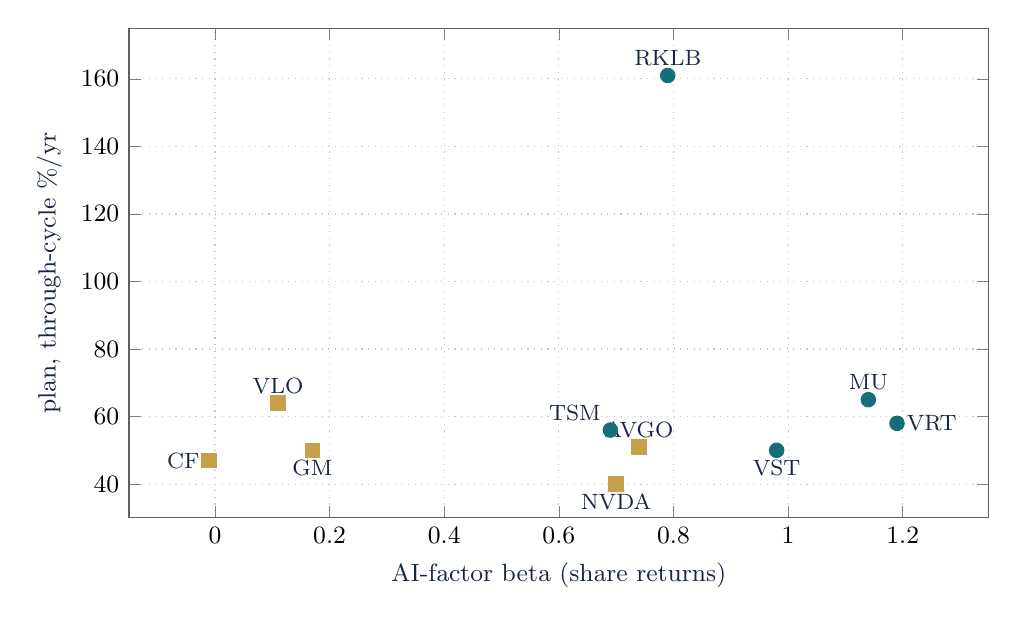
\begin{tikzpicture}
\begin{axis}[width=12.5cm,height=7.8cm,
  xlabel={AI-factor beta (share returns)},
  ylabel={plan, through-cycle \%/yr},
  xmin=-0.15,xmax=1.35,ymin=30,ymax=175,
  grid=both, grid style={dotted,gray!45},
  tick label style={font=\small},
  label style={font=\small\color{bcnavy}},
  axis line style={bcgrey}]
% incumbents: teal circles
\addplot[only marks,mark=*,mark size=2.6pt,color=bcteal] coordinates
  {(0.79,161) (1.19,58) (1.14,65) (0.69,56) (0.98,50)};
% candidates: gold squares
\addplot[only marks,mark=square*,mark size=2.6pt,color=bcgold] coordinates
  {(0.11,64) (0.17,50) (-0.01,47) (0.74,51) (0.70,40)};
\node[above,font=\footnotesize\color{bcnavy}] at (axis cs:0.79,161) {RKLB};
\node[right,font=\footnotesize\color{bcnavy}] at (axis cs:1.19,58) {VRT};
\node[above,font=\footnotesize\color{bcnavy}] at (axis cs:1.14,65) {MU};
\node[above left,font=\footnotesize\color{bcnavy}] at (axis cs:0.69,56) {TSM};
\node[below,font=\footnotesize\color{bcnavy}] at (axis cs:0.98,50) {VST};
\node[above,font=\footnotesize\color{bcnavy}] at (axis cs:0.11,64) {VLO};
\node[below,font=\footnotesize\color{bcnavy}] at (axis cs:0.17,50) {GM};
\node[left,font=\footnotesize\color{bcnavy}] at (axis cs:-0.01,47) {CF};
\node[above,font=\footnotesize\color{bcnavy}] at (axis cs:0.74,51) {AVGO};
\node[below,font=\footnotesize\color{bcnavy}] at (axis cs:0.70,40) {NVDA};
\end{axis}
\end{tikzpicture}
\end{center}
\tabnote{The admission picture: teal circles are incumbents, gold squares are
candidates. The book's risk lives on the right; the additions worth having sit on
the left at incumbent-grade plans.}

\section{The decision}

\textbf{Admit GM, VLO and CF.} Tested 55--138\% with AI betas of 0.0--0.17, book
correlations of 0.0--0.24 and name-level drawdowns of 11--17\% against the
incumbents' 17--40\%.

\begin{center}
\begin{tabular}{lrrrr|r}
\toprule
 & full \%/yr & full maxDD & test \%/yr & test maxDD & Jan--Apr 25 \\
\midrule
five (current)       & 84.8\% & 39.3\% & 122.4\% & 29.6\% & $-18.7\%$ \\
eight ($+$GM/VLO/CF) & 71.4\% & 29.7\% & 101.9\% & 20.1\% & $-11.8\%$ \\
\bottomrule
\end{tabular}
\end{center}

\tabnote{Held construction, common calendar, verified fills. The last column is
the strategy loss through the one AI drawdown in sample.}

About 13 points of book return buys 10 points of drawdown and a third off the
stress loss --- the trade the June study measured, confirmed here on the verified
instrument.

\textbf{Decline NVDA and AVGO} (judged purely on the numbers --- the weekly book
has been withdrawn). Plans of 40\% and 51\% with AI betas of 0.70--0.74 and book
correlations of 0.3--0.4: at equal weight a new name takes capital from what it
dilutes, and these two would lower the book's return without lowering its risk.
AVGO adds the second-worst fragility check in the table and a reference vector
fitted in this session.

\textbf{VST is flagged, not actioned}: lowest tested return (46.2\%), highest AI
beta (0.98), collapsing fresh fits. If the eight-name allocation ever needs a
funding source, it is the candidate.

\textbf{Implementation}, per the standing open item: eight names at 12.5\% each,
floor and cap both 0.125; Feed/Model/Dashboard/blotter rows for the three
additions; \texttt{IBKR\_Orders} widened to cover 16 sleeves. Planning figures for
the additions stay at the June levels (GM 33\%, VLO 35\%, CF 41\%), which the new
tested numbers are consistent with; VLO's 137.9\% tested half is one energy rally
and is not to be planned on.

\section{The eight-name book}

The book as it stands after admission, all figures on the verified basis:

\begin{center}
\begin{tabular}{lrrrr}
\toprule
 & plan & trades/yr & AI $\beta$ & corr to five-book \\
\midrule
TSM  &  56\% &  92 & 0.69 & 0.47 \\
VRT  &  58\% &  74 & 1.19 & 0.48 \\
VST  &  50\% &  78 & 0.98 & 0.35 \\
RKLB & 161\% & 118 & 0.79 & 0.94 \\
MU   &  65\% &  57 & 1.14 & 0.59 \\
GM   &  50\% &  61 & 0.17 & 0.24 \\
VLO  &  64\% &  35 & 0.11 & 0.04 \\
CF   &  47\% &  27 & $-0.01$ & $-0.01$ \\
\midrule
\textbf{average / total} & \textbf{69\%} & \textbf{542} & \textbf{0.63} & \textbf{0.39} \\
\bottomrule
\end{tabular}
\end{center}

\tabnote{Plan is each name's full-sample through-cycle verified return; the average
is the simple mean --- the held construction (equal capital, compounding
independently) gives \textbf{71.4\%/yr} for the eight-name book. Trades/yr is the
average verified buy count per year; the bottom row is the book's \emph{total},
$\approx$542 fills a year, about 2.2 per session across the sixteen sleeves. Correlations are measured against
the \emph{current five-name} book on the tested half, so the incumbents' values
partly reflect self-correlation; the candidates' values are the clean read.}

\subsection{The book's weighting to the AI trade after admission}

The current five-name book is the AI trade five-for-five: every dollar sits in an
AI-adjacent name, and the capital-weighted AI beta is \textbf{0.96}. After
admission, five names in eight --- 62.5\% of capital --- carry that exposure, and
the book's average beta falls to \textbf{0.63}, roughly a third off. The three
additions hold 37.5\% of capital at betas of $-0.01$ to $0.17$. On strategy
returns, where the sleeves are in cash almost half the time, the measured effect is
the June study's: book beta $0.58 \to 0.41$, full-sample drawdown
$39.3\% \to 29.7\%$, and the Jan--Apr 2025 stress loss $-18.7\% \to -11.8\%$.

Three honest qualifications. First, the AI factor remains the book's single
dominant risk --- the additions scale that risk down by about a third; they do not
change what the risk \emph{is}. A deep AI drawdown still sets the book's worst
week. Second, the concentration apex is untouched: RKLB carries a 0.94 correlation
to the book, the largest plan in the table, and a parameter vector no fresh fit can
recover --- the single-name risk the eight-name structure dilutes least. Third, VLO
and CF share the energy complex (0.41 correlation between them), so the three
additions contribute nearer two-and-a-half independent names than three.

\vspace{0.5cm}
{\color{bcnavy}\hrule height 0.8pt}
\vspace{0.2cm}
{\footnotesize\color{bcgrey} Reproduction: \texttt{premarket\_study/} ---
\texttt{fresh\_opt.py} (protocol and variants), \texttt{fresh\_opt\_cands.py}
(candidate sweep), \texttt{rank\_book.py} (ranking), \texttt{rolling\_mle.py} and
\texttt{mle\_homogeneity.py} (drift study), \texttt{live5\_load.py} (workbook
mirror check), \texttt{minute\_index.py} (5-minute fill verification). Derived
data and price extracts are untracked by design.}

\end{document}
